\externaldocument{GEP/deliverable1.tex}

\section{Integración de OmpSs-2 en C/C++ COMPSs}

Con tal de realizar una buena integración necesitamos conocer bien cómo funcionan y/o cómo están hechos los componentes a integrar. Con tal de adquirir los conocimientos necesarios, vamos a indagar en la estructura interna del \textit{binding} de \textit{C/C++} de \textit{COMPSs} y a entender cómo se desarrolla y compila una aplicación. También deberemos ver cómo funciona la \textit{API} del \textit{runtime} de \textit{OmpSs-2} \textit{Nanos6} y el proceso habitual de desarrollo y compilado de una aplicación que utiliza el modo librería.

\subsection{Estructura de los bindings}

El \textit{runtime} de \textit{COMPSs} fue desarrollado en \textit{Java}, por lo que si queremos soportar cualquier lenguaje (salvo el propio \textit{Java}), necesitamos de alguna manera establecer comunicación con ese lenguaje. Es decir, necesitaremos un mecanismo que nos permita ejecutar código de este lenguaje a soportar, por supuesto, en ambas direcciones. 
\par\bigskip
Actualmente, \textit{COMPSs} cuenta con los \textit{bindings} de \textit{C/C++} y \textit{Python} (usualmente conocido como \textit{PyCOMPSs}), que utilizan estos mecanismos descritos anteriormente. Para efectuar la ejecución entre \textit{Java} y \textit{C/C++} se utiliza la \textit{Java Native Interface}, dado que desde \textit{Python} se puede utilizar la \textit{Python-C API} para , con un componente intermedio entre \textit{Python} y \textit{Java} escrito en \textit{C/C++} (utilizando la \textit{JNI}) permitiríamos efectuar llamadas desde \textit{C/C++} y \textit{Python} al \textit{runtime} y al revés. 
\par\bigskip
La siguiente imagen muestra la estructura general de los \textit{bindings} actuales. Las cajas representan componentes de la arquitectura, el color de cada caja ha sido escogido para representar un lenguaje, por lo que dos cajas del mismo color que estén conectadas directamente con un flecha no requieren de mecanismos adicionales.

\begin{figure}[H]
    \centering 
    \caption{Estructura de los bindings de COMPSs.}
    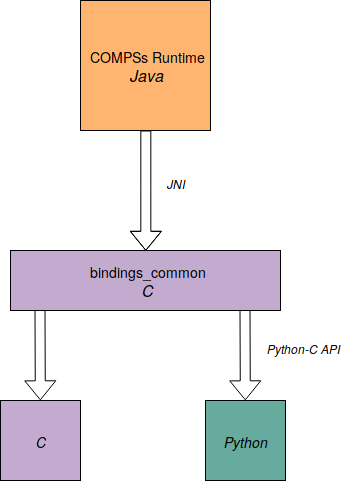
\includegraphics[scale=0.6]{estructuraBindings.png}
    \label{fig:estructura_bindings}
\end{figure}

\subsection{Modelo de ejecución en el binding C/C++}
\label{sec:bindings}

\textit{C} y \textit{C++} son lenguajes de programación compilados, esto quiere decir que necesitamos un segundo programa llamado compilador que procese nuestro programa y genere un fichero que nuestro ordenador pueda ejecutar, a este proceso se le llama compilar y al fichero generado, binario. De esta manera, para poder obtener el modelo de ejecución introducido en la sección \ref{modeloejecucion}, necesitaremos compilar dos binarios, uno para el \textit{master} y otro para los \textit{workers}.
\par\bigskip

\begin{comment}
La aplicación que desarrolla el usuario, \textit{a priori} no envía las tareas a ejecutar ni las dependencias entre estas, no gestiona el \textit{runtime}, pero es desarrollada siguiendo unas directrices que nos permitirán generar código que sí gestione todo lo que es necesario con tal de que la aplicación se distribuya correctamente. 
\end{comment}

La aplicación que desarrolle el usuario, tiene que ser transparente al \textit{runtime}, para conseguirlo tan sólo se necesita una interfaz indicando las tareas a detectar al ejecutar la aplicación. Entonces, una vez compilemos la aplicación de COMPSs en C/C++, se generará automáticamente (a partir de ahora \textit{autogenerar}) código para las tareas, que gestionarán la comunicación con el \textit{runtime}.
\smallskip
La siguiente imagen describe de manera visual cómo se compila una aplicación. 

\begin{figure}[H]
    \centering 
    \caption{Proceso de compilación de una aplicación COMPSs C/C++.}
    %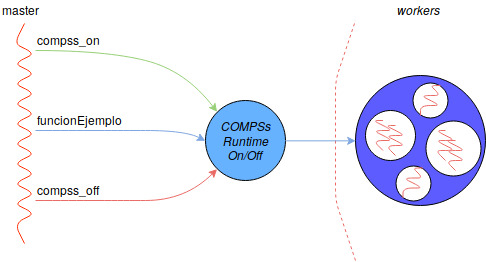
\includegraphics[width=\textwidth]{sta-masterworker.jpg}
    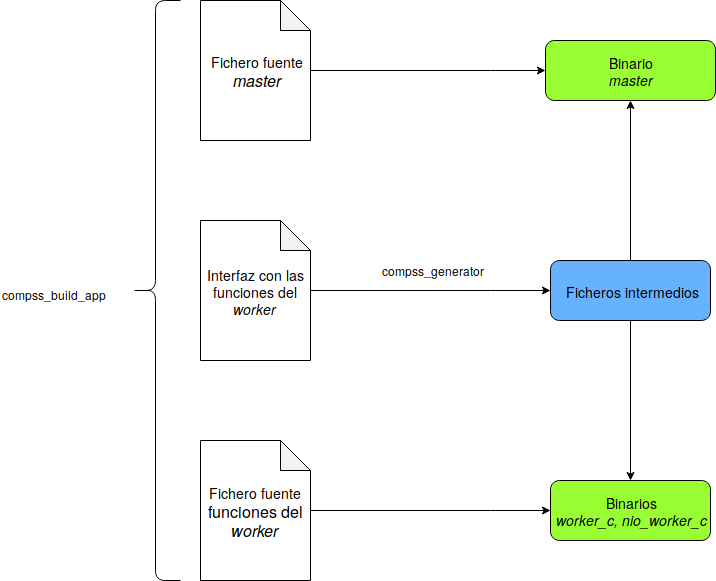
\includegraphics[scale=0.6]{workflowCompilado.png}
    \label{fig:workflowcompilado}
\end{figure}

\par\bigskip
Para facilitar el compilado de la aplicación se utiliza el script \textit{compss\_build\_app}, y para hacer la generación de código a partir de la interfaz, el binario \textit{compss\_generator}.
La aplicación una vez desarrollada por el usuario, compilada sin \textit{COMPSs} por el medio también funcionaría, pero sencillamente las tareas serían ejecutadas \textit{in situ} en el \textit{master}.  Lo que pretendemos hacer al introducir \textit{COMPSs} es que el \textit{master}, en vez de ejecutar la tarea, comunique al \textit{runtime} que se debe ejecutar una tarea, y este se encargue de ejecutarla en un \textit{worker}, todo evidentemente, de manera transparente al usuario.
\par\bigskip

\bigskip
En la figura \ref{fig:workflowcompilado} veíamos la caja negra de ficheros intermedios, estos ficheros son el \textit{stubs} y \textit{executor} (siempre del estilo, \textit{ejemplo-stubs.cc} y \textit{ejemplo-executor.cc} donde ejemplo es el nombre de la aplicación compilada). El fichero \textit{stubs} corresponde con la parte del \textit{master} que se encargará de comunicarse con el \textit{runtime} para registrar la tarea. Esto lo consigue implementando las funciones de las tareas con el código para gestionar su registro, es decir, sustituyendo el código que sería propio de la ejecución de cada tarea por un código para efectuar el registro en el \textit{runtime}. Una vez registrada la tarea, eventualmente el \textit{runtime} designará a un \textit{worker} a ejecutarla. El \textit{worker} recibirá la tarea que debe ejecutar, los datos necesarios y más parámetros, el \textit{executor} ha sido \textit{autogenerado} con el código principal de la aplicación, por lo que conoce como gestionar los datos y parámetros recibidos para ejecutar la tarea pertinente. 

\begin{comment}
\begin{figure}[H]
    \centering  
    \caption{Registro y ejecución de tareas en una aplicación COMPSs C/C++.}
    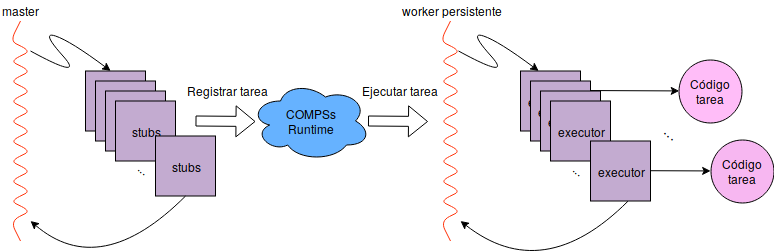
\includegraphics[scale=0.6]{stubs-executor.png}
    \label{fig:stubs-executor}
\end{figure}

La imagen anterior muestra las llamadas a funciones pertinentes a \textit{stubs} que contienen el código para registrar las tareas en el \textit{runtime}, la eventual ejecución de las tareas registradas en los \textit{workers} que haya disponibles y como toma parte su ejecución mediante el \textit{executor}. Ahora que sabemos como se estructura un \textit{binding}, y en concreto, como funciona el de \textit{C/C++}, el siguiente paso es estudiar el funcionamiento de \textit{OmpSs-2}.

%\subsection{Conceptos básicos de OmpSs-2}

\subsubsection{Mercurium}

\textit{Mercurium} es el encargado de compilar una aplicación de \textit{OmpSs-2} y hacer que las directivas insertadas en el código tengan efecto sobre este. De manera superficial, lo que hace es añadir código para gestionar el \textit{runtime}, encender el \textit{runtime}, añadir las tareas, notificar las dependencias y un largo etcétera. 

\subsubsection{Nanos6}

\todo{Pensar algo}
\end{comment}

\subsection{Modo librería: nanos6\_spawn\_function \label{spawnfunction}}

En la sección \ref{sec:bindings} dimos una visión más interna y propia de desarrollador del \textit{binding} de \textit{C/C++}. Sobre \textit{OmpSs-2} necesitamos saber, como se desarrolla una aplicación, en concreto con el modo librería.
\medskip

Esta funcionalidad, nos permite registrar una tarea en el \textit{runtime} de \textit{OmpSs-2} de manera asíncrona, con lo cuál podremos brindar a cada tarea y sus sucesoras un entorno aislado del resto. Gracias a esto, conseguiremos arreglar el problema con la migración de \texit{threads}, planteado en la sección \ref{compssompss}. \smallskip

\begin{lstlisting}[caption={Definición de la función nanos6\_spawn\_function.},captionpos=b, label={lst:nanos6spawn}, language=C++]
void nanos6_spawn_function(
   void (*function)(void *), 
   void *args,
   void (*completion_callback)(void *), 
   void *completion_args, 
   char const *label
);
\end{lstlisting}

La anterior imagen muestra la definición de la función que nos permitirá registrar una función \textbf{function} con argumentos \textbf{args} en el \textit{runtime}. Una vez ejecutada la función registrada como tarea, se ejecutará la función \textbf{completion\_callback} con argumentos \textbf{completion\_args} (mecanismo conocido como \textit{callback}, de ahí el nombre), el argumento de la función \textit{label} sirve para etiquetar la tarea con el nombre que contenga.

\subsubsection{Ejemplo}

Con tal de entender como funciona un programa que utilice el modo librería, vamos a ver un ejemplo sencillo. Este programa de ejemplo, hará \textit{spawn} de una función y dentro de ésta se generarán tareas con dependencias entre ellas. \smallskip

\begin{lstlisting} [caption={Función a ser registrada como tarea.},captionpos=b, label={lst:nanos6\_ejemplo}, language=C++]
 int nanos6_ejemplo(int* a) {

    int local_a;

    #pragma oss task shared(local_a) out(local_a) 
    {
        local_a = a[0];
    }

    #pragma oss task shared(local_a) inout(local_a)
    {
        local_a = local_a * 4;
    }

    #pragma oss taskwait

    return local_a;
}
\end{lstlisting}

En la imagen podemos ver la función \textbf{nanos6\_ejemplo}, ésta tiene como parámetro un puntero a enteros \textbf{a} y retorna un valor del tipo \textbf{int}. La función será registrada como tarea desde otro fichero. El cálculo que se realiza en la función no tiene la menor importancia, es solo un \textbf{ejemplo}. \medskip

Por supuesto, esta función será compilada con \textit{Mercurium}, si no fuera el caso, la función se ejecutaría correctamente pero no se generarían las tareas de dentro de la función, por lo cuál la ejecución sería secuencial. 

\begin{lstlisting} [caption={Gestión del modo librería desde el main.},captionpos=b, label={lst:library-main}, language=C++]
    char const *error = nanos6_library_mode_init();
    if (error != NULL)
    {
        fprintf(stderr, "Error initializing Nanos6: %s\n", error);
        return 1;
    }

    condition_variable_t cond_var = COND_VAR_INIT;

    ejemplo_wrapper_args_t args;

    int A = 1;
    args.array = &A;
    
    nanos6_spawn_function(ejemplo_wrapper, &args, 
    condition_variable_callback, &cond_var, 
    "spawned ejemplo");

    wait_condition_variable(&cond_var);

    printf("%li\n", args.ret);

    nanos6_shutdown();

\end{lstlisting}

Las funciones \textit{nanos6\_library\_mode\_init()} y \textit{nanos6\_shutdown()} efectúan respectivamente el encendido y apagado del \textit{runtime}, el código que vemos entre estas dos llamadas es el correspondiente para registrar una función como tarea utilizando el modo librería. Dado que la función nanos6\_spawn\_function espera como un puntero los parámetros a pasar a la función, se deben incluir todos dentro de una estructura que los pueda contener, el \textit{struct} \textit{ejemplo\_wrapper\_args\_t} tiene los campos \textbf{a} y \textbf{ret} que corresponden al parámetro de la función \textit{nanos6\_ejemplo} y valor de retorno de ésta.

\bigskip
Un detalle que no se ha comentado es que la ejecución de este código será efectuada por \textit{pthreads}, el estándar \textit{POSIX} de \textit{threads}. Dado que la ejecución de la tarea tendrá lugar de manera \textbf{asíncrona} es necesario un mecanismo de sincronización, la implementación de \textit{threads} que utilizamos (y por tanto los mecanismos de sincronización dependerán de estos) es la explicada en el apéndice \ref{appendix:pthread}.

\bigskip

Como es necesario utilizar una estructura auxiliar para pasar los parámetros mediante un puntero, necesitaremos también una función intermedia con la cuál llamar a la función que realmente queremos registrar como tarea. Habitualmente a este tipo de funciones intermedias se les llama \textit{wrapper}. En la siguiente imagen veremos la función que actúa como \textit{wrapper} de la función \textit{nanos6\_ejemplo}. \smallskip

\begin{lstlisting} [caption={Wrapper de la función nanos6\_ejemplo.},captionpos=b, label={lst:library-wrapper}, language=C++]
 void ejemplo_wrapper(void *untyped_arg)
{
    ejemplo_wrapper_args_t *args = 
        (ejemplo_wrapper_args_t *) untyped_arg;
    args->ret = nanos6_ejemplo(args->a);
}
\end{lstlisting}

El puntero de tipo \textit{void} puede contener cualquier tipo de estructura, aprovechando que sabemos que únicamente deberá contener el tipo \textit{ejemplo\_wrapper\_args\_t} se hace un \textit{cast} para interpretarlo como la estructura deseada. Se asigna \textbf{ret} al valor de retorno y se pasa \textbf{a} como parámetro.

\todo{faltan detalles de compilado...}

\subsection{Integración}

\todo{TODO}

Ahora que tenemos claro el funcionamiento de ambas partes, podemos plantear un prototipo de la integración e implementarlo. Está claro que \textit{OmpSs-2} tomará parte únicamente en los nodos del tipo \textit{worker}, ya que es dónde realmente se ejecutarán las tareas detectadas por el \textit{master}. Entonces, si 

%En los apartados se ha visto cómo funciona una aplicación de \textit{COMPSs} en \textit{C/C++}, y por otra parte como funciona \textit{OmpSs-2} y el modo librería con la función \textit{nanos6\_spawn\_function}. Para tener una integración funcional nos bastará con activar el modo librería en los \textit{workers} de \textit{COMPSs}, añadir código para registrar las tareas de \textit{COMPSs} en el \textit{runtime} de \textit{OmpSs-2} utilizando \textit{nanos6\_spawn\_function} y añadir los mecanismos necesarios para esperar a la finalización de estas. 

\section{Aplicación COMPSs+OmpSs-2}



\section{Estudio del rendimiento}































